\documentclass[pdf]{beamer}

\usetheme{Median}

\usepackage{graphicx}
\usepackage{pgfpages}
\usepackage{caption}
\usepackage{amsmath}
\usepackage{tensor}
\usepackage{tikz}
\usepackage{pgfplots}
\setbeameroption{show notes}


\newcommand{\credit}[1]{\tiny{\textcolor{blue}{Credit: #1}}}




\title[Stochastic signal originating from CGBs mesured by LISA]{Characterization of the stochastic signal originating from compact binary
populations as measured by LISA}
\subtitle{Nikolaos Karnesis et al}
\author{MohammadReza Torkamani}

\begin{document}
\setbeamertemplate{caption}{\raggedright\insertcaption\par}

\begin{frame}
    \titlepage
\end{frame}

\begin{frame}{Table of Contents}
\vspace*{.1cm}
  \tableofcontents
\end{frame}
\section{Introduction}
\subsection{Gravitational waves}
\begin{frame}{Gravitational waves}
 \begin{columns}
 	\hspace{.5cm}
    \column[c]{0.5\textwidth}
    Ripples in space-time caused by accelerated masses.
        
	
	\begin{block}{Einstein field equations}
	\begin{equation*}
    \tensor{G}{_\mu_\nu} = \dfrac{8\pi G}{c^4} \tensor{T}{_\mu_\nu}  
    \end{equation*}
	\end{block}
	
	
    \begin{equation*}
    \tensor{g}{_\mu_\nu} = \tensor{\eta}{_\mu_\nu} + \tensor{h}{_\mu_\nu} \qquad |h|<<1 
    \end{equation*}
    \begin{equation*}
    \tensor{\bar{h}}{_\mu_\nu} = \tensor{h}{_\mu_\nu} -\dfrac{1}{2} \tensor{\eta}{_\mu_\nu} h  
    \end{equation*}
    
    
    \column{0.5\textwidth}
    \begin{figure}
    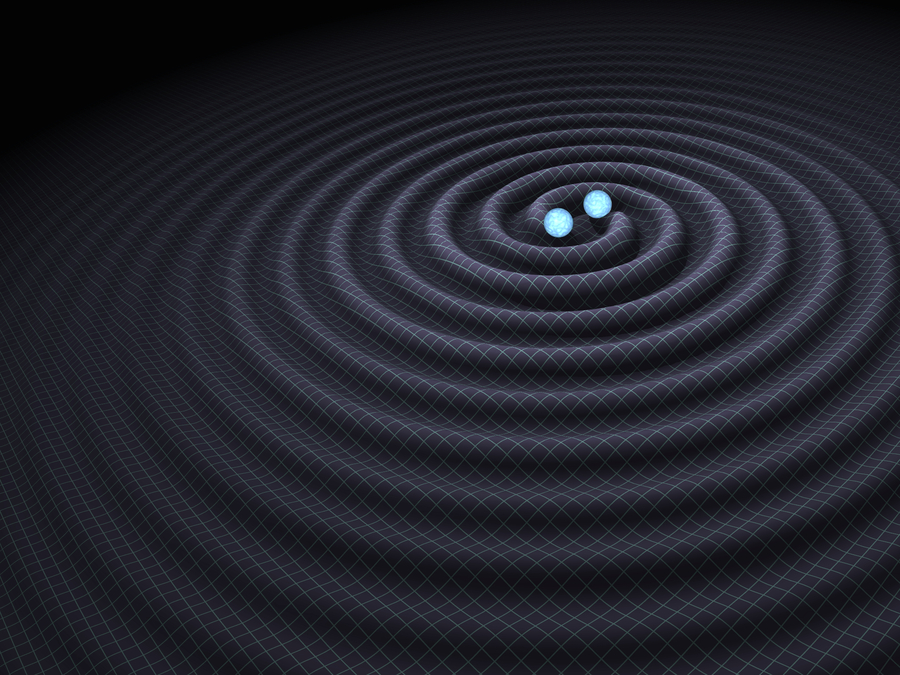
\includegraphics[scale=.14]{fig/GravWave.jpg}
    \caption*{\credit{R. Hurt (Caltech-IPAC)}}
    \end{figure}
  \end{columns}

\end{frame}

\begin{frame}{Gravitational waves}

	\begin{columns}
	\hspace{.5cm}
	\column[c]{0.5\textwidth}
	Lorenz gauge: $\partial_\mu \tensor{\bar{h}}{^\nu^\mu} = 0$
	\begin{block}{Wave equation}
	\begin{equation*}
	\Box \tensor{\bar{h}}{_\mu_\nu} = 0
	\end{equation*}		
	\end{block}
	
	\begin{equation*}
	\tensor{\bar{h}}{_\mu_\nu} = \tensor{A}{_\mu_\nu} \exp{(ik_\alpha x^\alpha)}
	\end{equation*}
	
	Transverse traceless gauge: $\tensor{\bar{h}}{_\mu_\nu} U^\mu = 0$ and $\tensor{\bar{h}}{_\mu^\mu} = 0$
	
	\column[c]{0.5\textwidth}
	
	\begin{align*}
	16 \xrightarrow{symetry} 10 \xrightarrow[gauge]{Lorenz} 6 \xrightarrow[gauge]{TT} 2
	\end{align*}		
	\begin{equation*}
	\tensor{h}{_\mu_\nu} = \begin{bmatrix}
	0&0&0&0\\
	0&h_+&h_\times&0\\
	0&h_\times&-h_+&0\\
	0&0&0&0
	\end{bmatrix}
	\end{equation*}		
	
\begin{figure}
 \scalebox{.5}{
\begin{tikzpicture}
  \begin{axis}[
    % Comment out or remove the following lines to hide the axes
    hide axis,
    ticks=none,
  ]

  % Plane 1
  \addplot3[fill=blue, opacity=.5, mesh, domain=-5:5, y domain=-5:5]
    {0};

  % Plane 2
  \addplot3[fill=red, opacity=.5, mesh, domain=-5:5, y domain=-5:5]
    {1};

  % Plane 3
  \addplot3[fill=green, opacity=.5, mesh, domain=-5:5, y domain=-5:5]
    {2};


	\draw[->, thick] (300,300,0) -- (300,300,260) node[above, right] {$U^\mu$};
  \end{axis}
  
\end{tikzpicture}}
\end{figure}		
	
	\end{columns}

\end{frame}

\subsection{Ground-based observatories}
\begin{frame}{LIGO Structure}
Giant Michelson interferometer
\begin{columns}
\column[c]{0.5\textwidth}
\begin{figure}
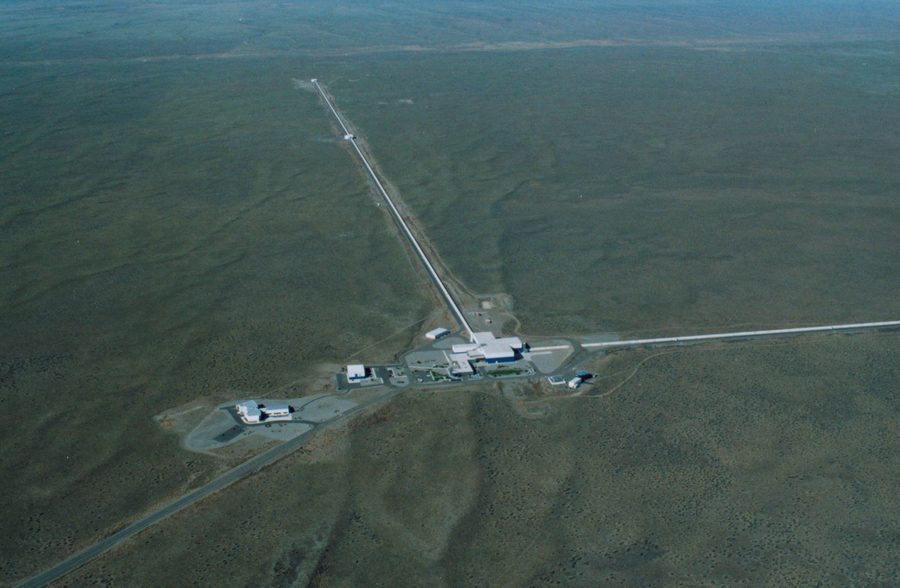
\includegraphics[scale=.6]{fig/HiResHanford_5.jpg}
\caption*{\credit{Caltech/MIT/LIGO Lab}}
\end{figure}
\column[c]{0.5\textwidth}
\begin{figure}
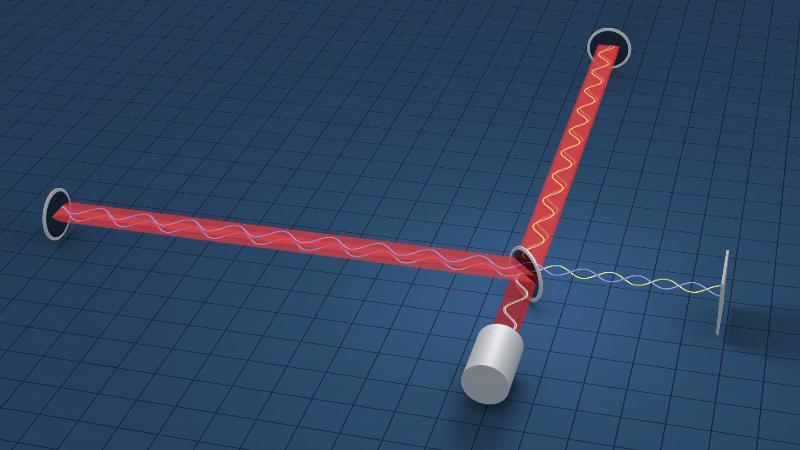
\includegraphics[scale=.14]{fig/IFO_SCHEME.png}
\caption*{\credit{D. V. Martynov et all, 2018}}
\end{figure}
\end{columns}
\begin{equation*}
S(t) = h(t) + n(t)
\end{equation*}
\end{frame}

\begin{frame}{LIGO Noise budget}
\begin{columns}
\column[c]{.65\textwidth}
\begin{figure}
\caption*{Hanford detector}
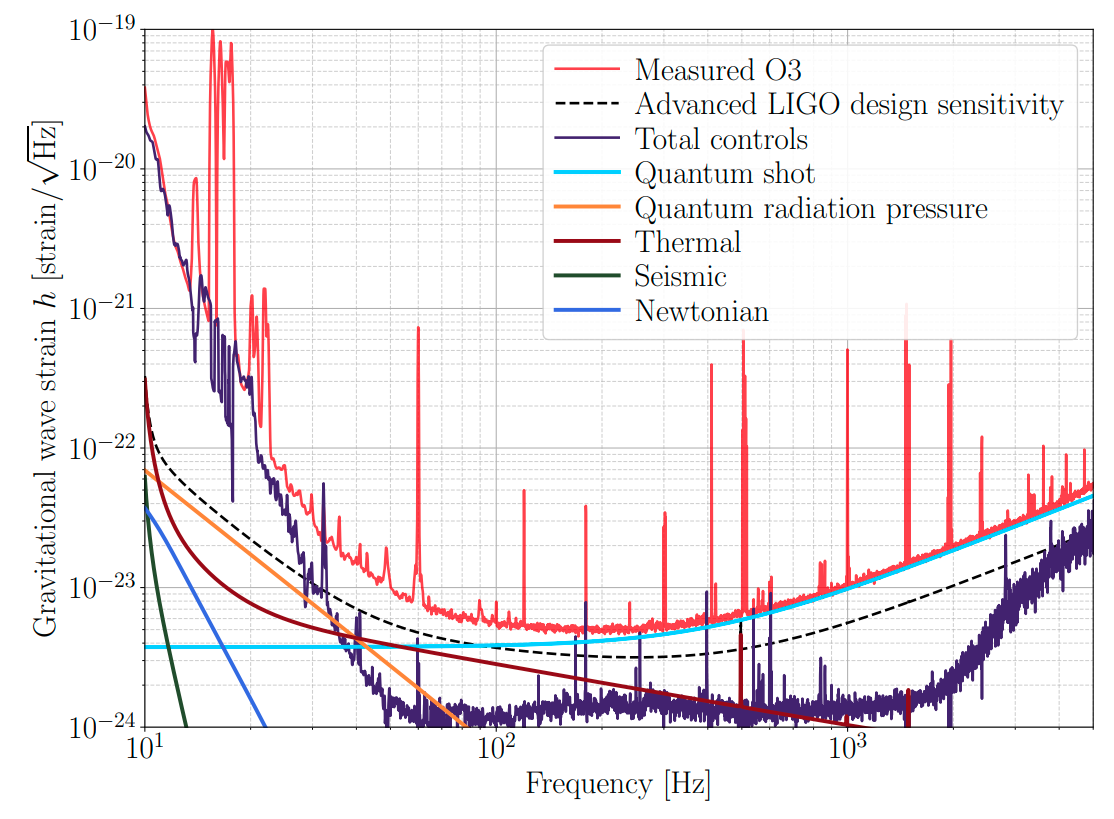
\includegraphics[scale=.17]{fig/noise-budget-ligo.png}
\caption*{\credit{Craig Cahillane et all, 2022}}
\end{figure}
\column[c]{.35\textwidth}

Dominant noise:

\begin{itemize}
\item  
Quantum shot in high frequency

\item  
seismic noise in low frequency
\end{itemize}

\end{columns}
\end{frame}

\begin{frame}{First detection}
\begin{figure}
\caption*{GW150914}
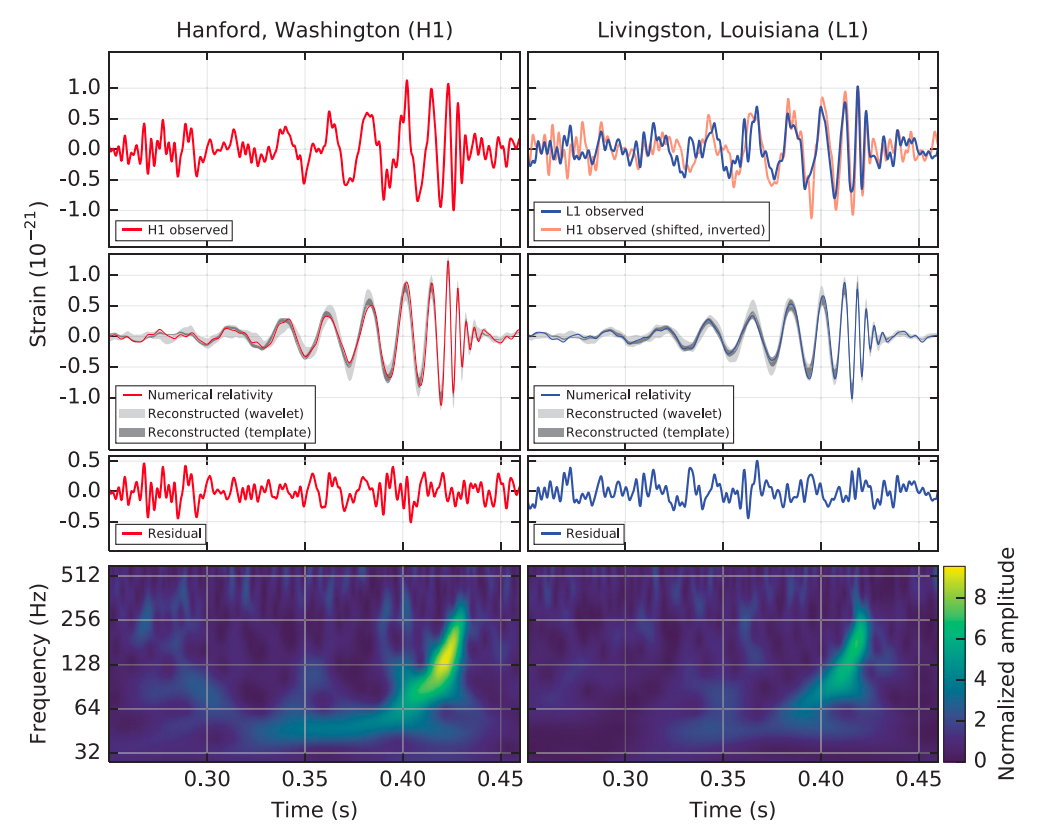
\includegraphics[scale=.17]{fig/GW150914.png}
\caption*{\credit{B. P. Abbott et al., 2016}}
\end{figure}
\end{frame}

\subsection{LISA}
\begin{frame}{Laiser Interferometer Space Antenna}
\begin{columns}

\column[c]{0.5\textwidth}
\begin{figure}
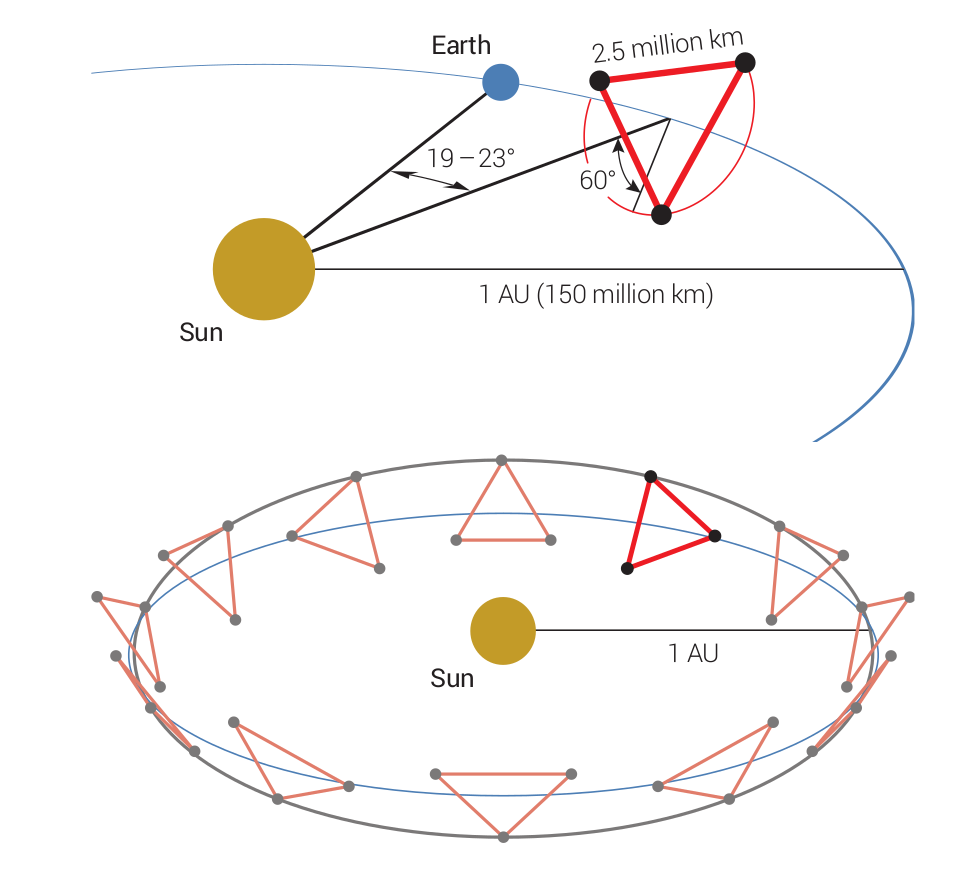
\includegraphics[scale=.15]{fig/LISA.png}
\caption*{\credit{Karsten Danzmann et al., 2017}}
\end{figure}

\column[c]{0.5\textwidth}
\begin{figure}
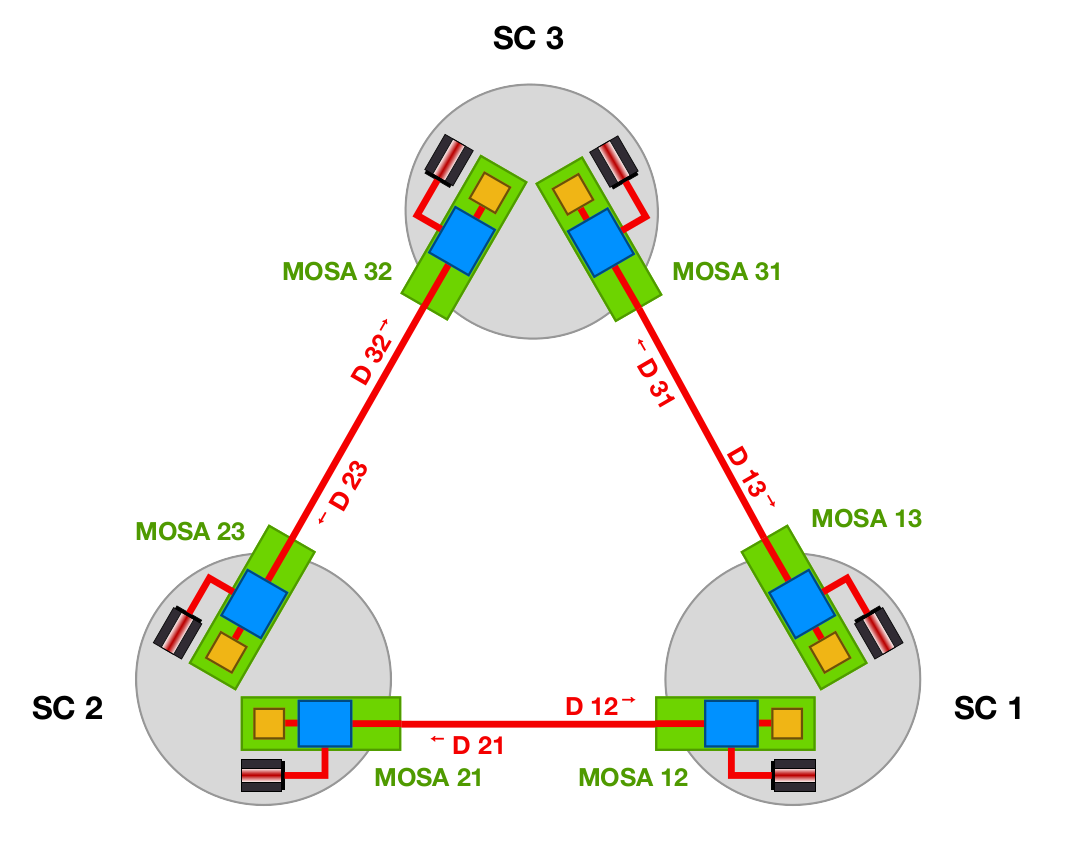
\includegraphics[scale=.12]{fig/LISAsch.png}
\caption*{\credit{Jean-Baptiste Bayle et al., 2021}}
\end{figure}

\end{columns}
\end{frame}

\begin{frame}{LISA Band}
\begin{columns}
\column[c]{0.5\textwidth}
\vspace{1cm}

\begin{figure}
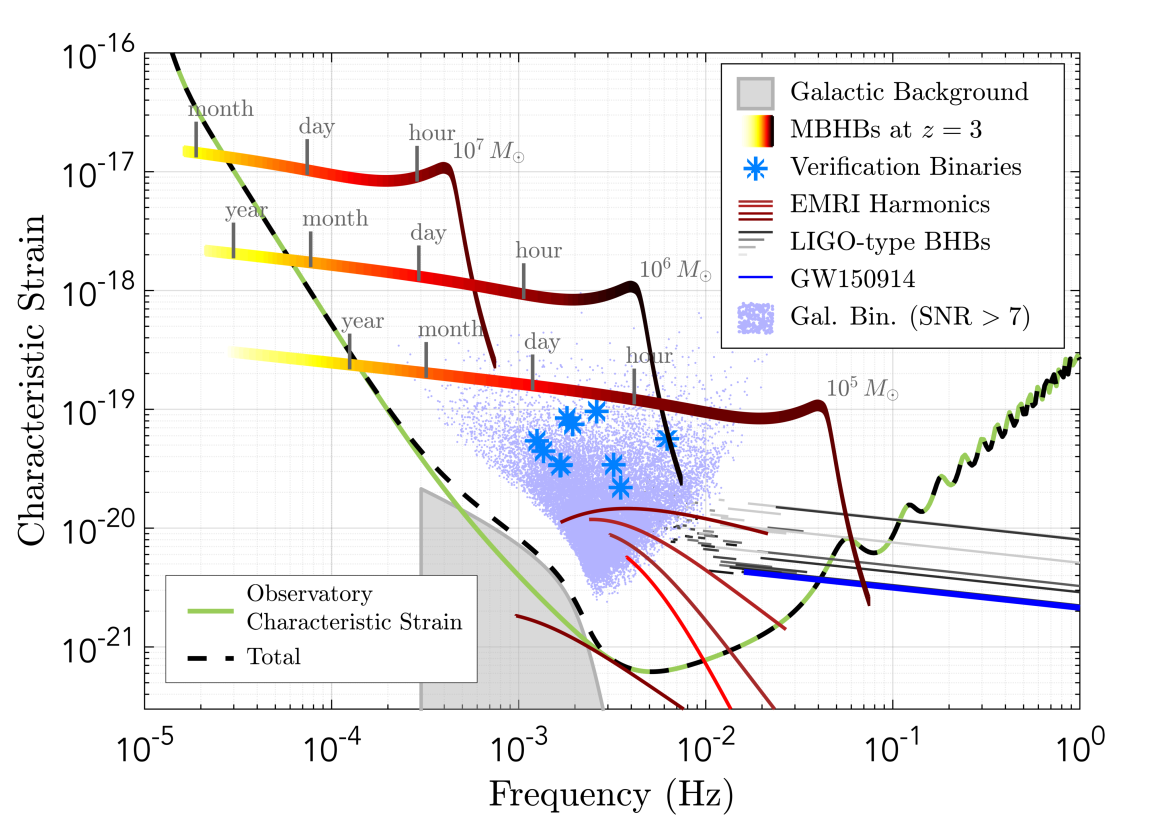
\includegraphics[scale=.13]{fig/observedLISA.png}
\caption*{\credit{Karsten Danzmann et al., 2017}}
\end{figure}
\column[c]{0.5\textwidth}
\vspace{1cm}

GW sources in LISA band
\begin{itemize}
\item Supermassive black hole binaries (SMBHBs)
\item Stellar-mass black hole binaries (SBBHs)
\item Ultracompact galactic binaries (CGBs)
\item extreme mass ratio inspiral (EMRIs)
\item stochastic GW background 
\end{itemize}
\end{columns}
\end{frame}

\begin{frame}{LISA Isuues}
\begin{itemize}
\item LISA data are expeted to be signal dominated
\item LISA sources are expected to be long-lived
\item GW signals will be overlapping in time(frequency)
\pause
\item Some signals can be resolvable due to high signal to noise ratio
\pause
\item remaining signals will affect the sensitivity as extra noise (confusion noise)
\end{itemize}
\end{frame}

%%%%%%%%%%%%%%%%%%%%%%%%%%
%%%%%%%%%%%%%%%%%%%%%%%%%%
\section{Methodology}
\begin{frame}{Overview}
\begin{itemize}
\item Simulating around 30 milion CGBs from Radler LISA data challenge dataset
\item Simulating the instumental noise using the LISA code simulatior
\item For each $T_{obs}$ gererate the idealized dataset in the frequency domain
\item Apply the method to find the final sensitivity
\item Fit the data with theoretical curve
\end{itemize}
\end{frame}

\begin{frame}{Methode}
\begin{itemize}
\item Assumpion: Bright sources with a signal-to-noise ratio larger than a given threshold are detected and charachterized without systematic bias or source cofusion.
\end{itemize}
\begin{block}{SNR}
\begin{align*}
\rho^2_{tot} &= \sum_k (h_k|h_k), \quad  \text{k:noise-orthogonal TDI variables} \\
h_k|h_k &= 4 \int_{0}^{\infty} df \dfrac{|\tilde{h}_k(f)|^2}{\tilde{S}_n(f)}, \quad \tilde{S}_n(f):\text{one-sided PSD} \\
\tilde{S}_n(f) &= \tilde{S}_{instr}(f) +\tilde{S}_{conf}(f)
\end{align*}
\end{block}
\end{frame}

\begin{frame}{Methode}
\begin{enumerate}
\item Simulating 30 milions CGBs
\item Calculating the PSD of the signal and the instrumental noise
\item Calculating the SNR of each source with respect to the instrumental noise ($\rho_i^{iso}$)
\item Stimating the SNR of each source using either a running mean or median on the power spectrum of the data ($\rho_i$)
\item If $\rho_i > \rho_0$ the source will be subtracted from the data
\item iterate the process
\end{enumerate}
\end{frame}

\section{Gravitational wave's detector}
\subsection{LIGO}
\begin{frame}
A
\end{frame}

\subsection{Interferometer}
\begin{frame}
A
\end{frame}

\subsection{Gravitational waves' detection}
\begin{frame}
A
\end{frame}

%\begin{frame}
%A
%\end{frame}

\section{Strain Sensitivity}
\begin{frame}{GW151226}
A
\end{frame}


\begin{frame}{Our Group}
A
\end{frame}

\section*{Reference}
\begin{frame}{Reference}
A
\end{frame}

\begin{frame}
\begin{center}
\Huge Thank you!
\end{center}
\end{frame}

\end{document}
